\subsection{Experiment}
The estimation problem is tested in Matlab Simulink. The experimental setup consists of the Open HRP3 simulator and the state estimator. The OpenHRP3 (Open Architecture Human-centred Robotics Platform version 3) is an integrated software platform for robot simulations and software developments \footnote{\url{http://www.openrtp.jp/openhrp3/en/about.html}}. It was developed as a cooperative work of University of Tokyo, General Robotix. Inc and National Institute of Advanced Industrial Science and Technology(AIST).

\begin{figure}
    \centering
    % We need layers to draw the block diagram
\pgfdeclarelayer{background}
\pgfdeclarelayer{foreground}
\pgfsetlayers{background,main,foreground}

% Define a few styles and constants
\tikzstyle{sensor}=[draw, fill=blue!20, text width=5em,text centered, minimum height=2.5em]
\tikzstyle{system} = [sensor, text width=6em, fill=green!30, 
    minimum height=12em, rounded corners]
\tikzstyle{input} = [coordinate]
\tikzstyle{sum} = [draw, fill=blue!20, circle, node distance=1cm]
%\tikzstyle{output} = [coordinate]
\def\blockdist{0.5}
\def\edgedist{0.75}
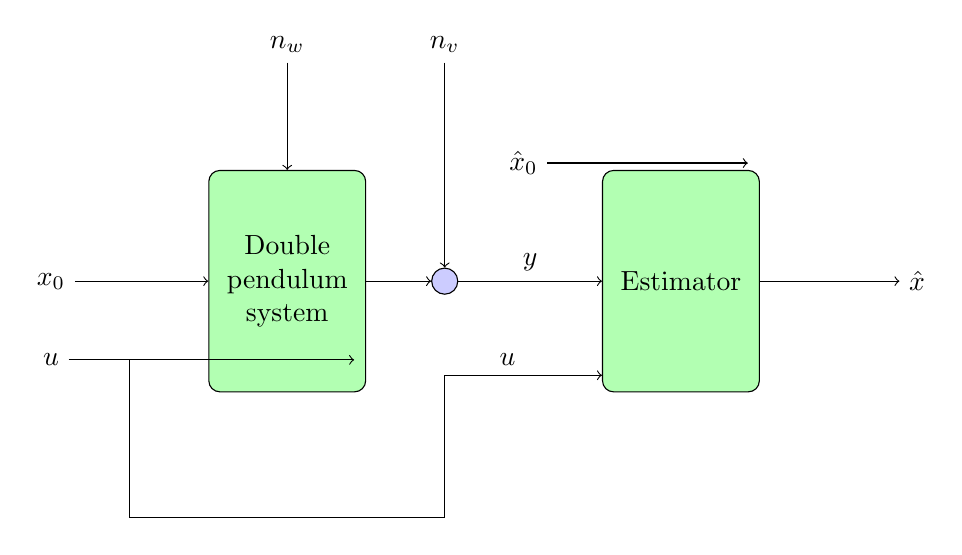
\begin{tikzpicture}
	% Define the nodes in the picture
	\node (sys_in)[yshift=1cm]{$x_0$};
	\node (u_in) [below of=sys_in,node distance=1cm]{$u$};
	\node (sys_u)[input,right of=u_in,node distance=1cm]{};
    \node (sim_sys) [system,right of=sys_in,node distance=3cm] {Double pendulum system};
    \node (sys_noise)[above of=sim_sys,node distance=3cm]{$n_w$};
    \node (msr_noise)[right of=sys_noise,node distance=2cm]{$n_v$};
    \node (msr_add)[sum,right of=sim_sys,node distance=2cm]{};
    \node (estimator) [system,right of=msr_add,node distance =3cm]{ Estimator};
    \node (est_in) [right of=sim_sys,node distance=3cm,yshift=1.5cm]{$\hat{x}_0$};
    \node (est_u) [input,right of =sim_sys, node distance=2cm,yshift=-3cm]{foo};
    \node (est_out)[right of=estimator,node distance=3cm]{$\hat{x}$};
    
    % Define the edges in the picture
    \draw [->] (sys_in) --node{}(sim_sys.west);
    \draw [-] (u_in) --node{}(sys_u);
    \draw [->] (sys_u) --node{}+(\edgedist,0);
    \draw [-] (sys_u) |-node{}(est_u);
    \draw [->] (est_u) |-node[pos=0.7,above]{$u$}(estimator.-130);
    \draw [->] (est_in) --node{}+(\edgedist,0);
    \draw [->] (sys_noise) --node{}(sim_sys.north);
    \draw [->] (msr_noise) --node{}(msr_add.north);
    \draw [->] (sim_sys.east) --node[above]{}(msr_add.west);
    \draw [->] (msr_add.east) --node[above]{$y$}(estimator.west);
    \draw [->] (estimator) --node{}(est_out);
\end{tikzpicture}
    \caption{Experimental setup of TORO}
\end{figure}

A rigid body algorithm is used in the estimator to compute dynamic $M(y_k), C(y_k,\dot y_k), g(y_k)$ and kinematic $J_r(y_k), J_l(y_k), H(y_k)$ parameters at time step $k$. An auto differentiation function that computes the derivative of the dynamic and kinematic parameters with respect to the the system states is integrated with the rigid body algorithm. 
\begin{figure}[h]
    \centering
    % We need layers to draw the block diagram
\pgfdeclarelayer{background}
\pgfdeclarelayer{foreground}
\pgfsetlayers{background,main,foreground}

% Define a few styles and constants
\tikzstyle{sensor}=[draw, fill=blue!20, text width=5em,text centered, minimum height=2.5em, rounded corners]
\tikzstyle{system} = [sensor, text width=5em, fill=green!30, 
    minimum height=8em]
%\tikzstyle{input} = [coordinate]
\tikzstyle{sum} = [draw, fill=blue!20, circle, node distance=1cm]
\tikzstyle{output} = [coordinate]
%\def\blockdist{0.5}
\def\edgedist{2.85}
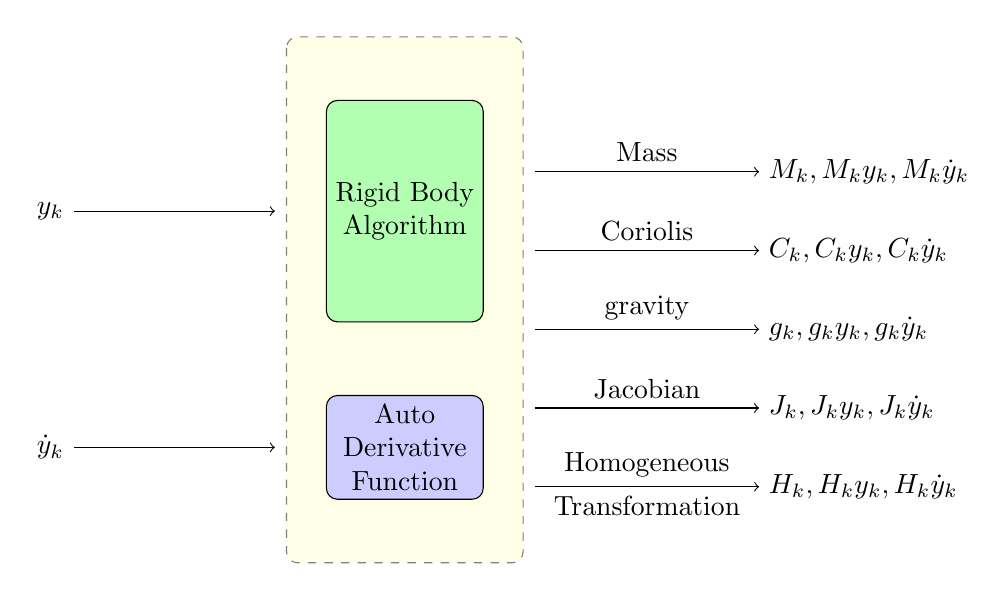
\begin{tikzpicture}
	% Define the nodes in the picture
	\node (y)[yshift=1cm]{$y_k$};
	\node (dy) [below of=y,node distance=3cm]{$\dot y_k$};
    \node (rigbdy_alg) [system,right of=y,node distance=4.5cm] {Rigid Body Algorithm};
    \node (auto_diff) [ sensor,below of=rigbdy_alg,node distance =3cm]{Auto Derivative Function};
    \node (M) [output,right of=rigbdy_alg,node distance=1.65cm,yshift=0.5cm]{};
    \node (C) [output,below of=M,node distance=1cm]{};
    \node (g) [output,below of=C,node distance=1cm]{};
    \node (J) [output,below of=g,node distance=1cm]{};
    \node (H) [output,below of=J,node distance=1cm]{};

    % Define the edges in the picture
    \draw [->] (y) --node{}+(\edgedist,0);
    \draw [->] (dy) --node{}+(\edgedist,0);
    \draw [->]  (M) --node[above]{Mass}+(\edgedist,0) node[right]{$M_k, \dfdx{M_k}{y_k},\dfdx{M_k}{\dot y_k}$};
    \draw [->]  (C) --node[above]{Coriolis}+(\edgedist,0) node[right]{$C_k, \dfdx{C_k}{y_k},\dfdx{C_k}{\dot y_k}$};
    \draw [->]  (g) --node[above]{gravity}+(\edgedist,0) node[right]{$g_k, \dfdx{g_k}{y_k},\dfdx{g_k}{\dot y_k}$};
    \draw [->]  (J) --node[above]{Jacobian}+(\edgedist,0) node[right]{$J_k, \dfdx{J_k}{y_k},\dfdx{J_k}{\dot y_k}$};
    \draw [->]  (H) --node[above]{Homogeneous} node[below]{Transformation}+(\edgedist,0) node[right]{$H_k, \dfdx{H_k}{y_k}, \dfdx{H_k}{\dot y_k}$};
    
    %Draw background layers
    \begin{pgfonlayer}{background}
        % Compute a few helper coordinates
        \path (auto_diff.west |- rigbdy_alg.north)+(-0.5,0.8) node (a) {};
        \path (auto_diff.south -| rigbdy_alg.east)+(+0.5,-0.8) node (b) {};
        \path[fill=yellow!10,rounded corners, draw=black!50, dashed]
            (a) rectangle (b);
    \end{pgfonlayer}
%\end{comment}
\end{tikzpicture}

    \caption{Structure of rigid body algorithm}
    \label{fig:luc_dyn}
\end{figure}
The Jacobian $J_k$ outputted by the algorithm shown in Figure \ref{fig:luc_dyn} is the body Jacobian of \emph{Toro's} right foot $J_r$ and left foot $J_l$ and homogeneous transformation matrix $H_k$ is the homogeneous transformation matrices of right foot $H_r$, left foot $H_l$ and floating base $H_b$ with respect to spatial frame(world frame).
The Jacobian matrices $A_k$ and $\hat C_{k+1}$ in Equations \ref{eq:sys_mat}, \ref{eq:msr_mat} are computed from the outputs in Figure \ref{fig:luc_dyn} as discussed in sections \ref{subsec:toro_predict} and \ref{subsec:toro_update}. The simulator and the estimator are driven by the same control inputs $u$. For instance the control inputs of \emph{Toro} are the torques applied to joints. The ground reaction forces $W_r$ and $W_l$ are measured in the simulator with the help of senor model of FTS. The ground reaction forces and the control torques are the input to prediction model in \ref{eq:toro_dis}.

The following scenario is simulated for the purpose of experiments. Initially \emph{Toro} is made to stand still on a floor (initial phase), after few seconds the robot is made to tilt around an edge by pushing it gently (tilting phase) and finally the robot is made to fall down by pushing it hard(falldown phase). During the tilting phase a force of low magnitude for short period of time is applied so the robot will not fall down.

Zero mean Gaussian noises $n_w$ and $n_v$ are added to the \underline{system or inputs} and measurements.
\begin{table}[H]
    \centering
    \begin{tabular}{|c|c|}
    \hline
    Noise &Variance \\ \hline
    \textbf{\underline{Process noise}} &\hspace{2mm}\\
    \hline
    \textbf{Measurement noise} &\hspace{2mm}\\
    Joint angles $q(rad)$ &$1e^{-6}$ \\ 
    Joint velocities $\dot q(rad/s)$ &$1e^{-4}$ \\
    Acceleration $\dot v^b(m/s^2)$ &$1e^{-2}$ \\ 
    Angular velocity $\omega^b(rad/s)$ &$1e^{-4}$ \\ \hline
    \end{tabular}
    \caption{Variance of simulated noises}
    \label{tab:toro_var}
\end{table}

The process $Q$ and measurement $R$ covariance matrices are set with the corresponding values of noise covariances given in Table \ref{tab:toro_var}. 
$$  \begin{aligned}
         Q &= diag();\\
         R &= diag([1e^{-6} \textbf{1}_{25,1}; 1e^{-4}\textbf{1}_{25,1}; 1e^{-2}\textbf{1}_{3,1};1e^{-4}\textbf{1}_{3,1}; 1e^{-12}\textbf{1}_{36,1} ]);,
     \end{aligned}$$
where $\textbf{1}_{r,c}$ is the matrix of dimesions $r \times c$ with all the elements as 1 [Appendix \ref{sec:symbols}]. The initial values of the estimator $\hat x_0$ and its covariace $P_0$ are 
$$ \begin{aligned} x_0 = \textbf{0}_{62,1}\\ P_0 = I_3, \end{aligned} $$  where $\textbf{0}_{62,1}$ is the zero matrix of dimensions $62 \times 1$ [Appendix \ref{sec:symbols}].
